%% ============================================================
%%  Urban Expansion Monitoring Using Transfer Learning on
%%  Historical Satellite Imagery
%%  IEEE Conference Format (IEEEtran)
%% ============================================================
\documentclass[conference]{IEEEtran}

%% ---- Packages -----------------------------------------------
\usepackage[T1]{fontenc}
\usepackage[utf8]{inputenc}
\usepackage{amsmath,amssymb,amsfonts}
\usepackage{graphicx}
\usepackage{booktabs}
\usepackage{multirow}
\usepackage{array}
\usepackage{xcolor}
\usepackage{hyperref}
\usepackage{cite}
\usepackage{balance}
\usepackage{subfig}
\usepackage{algorithm}
\usepackage{algorithmic}
\usepackage{url}
\usepackage{siunitx}
\usepackage[capitalise]{cleveref}
\usepackage{tikz}
\usetikzlibrary{shapes.geometric, arrows.meta, positioning}

\hypersetup{
  colorlinks=true,
  linkcolor=blue,
  citecolor=blue,
  urlcolor=blue
}

\graphicspath{{../outputs/figures/}}

%% ---- Document -----------------------------------------------
\begin{document}

%% ---- Title --------------------------------------------------
\title{Urban Expansion Monitoring Using Transfer Learning\\
on Historical Satellite Imagery}

\author{%
  \IEEEauthorblockN{Kaustubh Agarwal, Prajwal Gupta, Kabir Rai,
    P~Manideep Reddy, Naman Khurana, and Divyashree N}
  \IEEEauthorblockA{%
    \textit{Department of Computer Science and Engineering} \\
    \textit{PES University}, Bengaluru, India \\
    \{pes1ug23cs291, pes1ug23cs426, pes1ug23cs274, pes1ug23cs376\}@pesu.pes.edu \\
    pes1202201027@pesu.pes.edu, divyashreen@pes.edu}
}

\maketitle

%% ============================================================
%%  ABSTRACT
%% ============================================================
\begin{abstract}
Rapid, uncontrolled urban expansion in Indian metropolitan regions threatens legally protected ecological zones, yet existing studies largely rely on single-city, single-seed SVM/Random-Forest classifiers and stop short of forecasting or alerting. We present an end-to-end framework that unifies transfer-learning land-cover classification, SAR--optical fusion, self-supervised pre-training, uncertainty-aware forecasting, and regulatory encroachment alerting. Using Sentinel-2 imagery over Mumbai, Delhi~NCR, and Bangalore, we construct a benchmark of 2{,}730 patches under a novel three-class taxonomy (Urban, Non-Urban, Transition) auto-labelled from ESA WorldCover~2021, and evaluate six models across three random seeds. With three-stage progressive fine-tuning and a combined cross-entropy--focal--Dice loss, ResNet50 attains $97.5 \pm 0.2\%$ overall accuracy (OA)---six points above the best published Indian SVM (91.01\%); even an optimised SVM ($92.6\%$) trails deep learning by five points, confirming the gain is not an artefact of a weak baseline. We further introduce the first Leave-One-City-Out (LOCO) benchmark for Indian metros, which exposes a 15--20\% cross-city accuracy drop and a CNN--Transformer ranking reversal: Swin-Tiny generalises best to unseen cities ($79.1\%$) despite lower in-distribution accuracy than ResNet50 ($77.1\%$ LOCO). Finally, the classified maps drive an uncertainty-aware Bi-LSTM that forecasts urban area to 2035 with 95\% confidence intervals, and a rule-based engine that flags predicted encroachments on protected zones and routes them to the responsible authority (55 alerts in a seven-city simulation). All results are reported as mean$\pm$std over three seeds.
\end{abstract}

\begin{IEEEkeywords}
Urban expansion monitoring, transfer learning, Sentinel-2, SAR--optical fusion, self-supervised learning, Bi-LSTM forecasting, cross-city generalization, Indian metropolitan regions, regulatory encroachment alerts.
\end{IEEEkeywords}

%% ============================================================
%%  I. INTRODUCTION
%% ============================================================
\section{Introduction}

\subsection{Problem Domain}

India's urban population is projected to exceed 600~million by 2031, with major metropolitan regions already expanded two- to four-fold in built-up area since 1990~\cite{census2011}. This growth triggers three interlinked problems that ground inspection cannot solve. First, encroachment on legally protected zones continues despite the Coastal Regulation Zone Notification~2019~\cite{crz2019}, the Forest Conservation Act~1980~\cite{fca1980}, and the Wetland Rules~2017~\cite{wetland2017}; Mumbai's Sanjay Gandhi National Park, Bangalore's Bellandur wetland, and Delhi's Yamuna floodplain are routinely breached by informal construction. Second, infrastructure planning ignores uncertainty---point forecasts offer no confidence bounds, causing capital misallocation in Indian smart-city investments~\cite{smartcity}. Third, deep learning is under-used for Indian urban classification: backbones such as ResNet50~\cite{he2016}, EfficientNet~\cite{tan2019}, Swin~\cite{liu2021}, and MobileNetV3~\cite{howard2019} routinely exceed 97\% on European benchmarks~\cite{helber2019}, yet published Indian urban studies rely overwhelmingly on single-city SVM/RF pipelines reaching only 89--91\% OA~\cite{chamoli2024}, with no cross-city evaluation and no link from classification to forecasting or alerting. Cloud-masked Sentinel-2/1 and harmonized Landsat composites via Google Earth Engine (GEE) provide the coverage; what is missing is an integrated pipeline from raw Indian imagery to policy-actionable output.

\subsection{Key Contributions}

This paper contributes the following.
\begin{enumerate}
  \item \textit{Multi-city Indian urban expansion benchmark with the first LOCO evaluation for Indian metros.} We construct 2{,}730 Sentinel-2 patches across Mumbai, Delhi~NCR, and Bangalore (2017--2023), automatically labeled from ESA WorldCover~2021 with three classes (Urban, Non-Urban, Transition), and evaluate six models with three-seed statistical rigor (seeds 42, 123, 7).
  \item \textit{Progressive fine-tuning achieving ${97.5 \pm 0.2\%}$ OA} on real Indian data without any domain-specific pre-training, exceeding the best published Indian SVM benchmark~\cite{chamoli2024} by more than six points.
  \item \textit{Novel Transition class via morphological dilation} of urban boundaries (100\,m buffer), which models mixed-pixel ambiguity at the active urban--rural interface and is the class most relevant to encroachment detection.
  \item \textit{Uncertainty-aware Bi-LSTM forecasting} producing 95\% Monte-Carlo-Dropout confidence intervals on 2024--2035 urban-area forecasts---a capability absent from every published Indian urban forecasting study we surveyed.
  \item \textit{First weak-supervision-to-policy-action pipeline for Indian urban monitoring: classify $\to$ time series $\to$ forecast $\to$ regulatory alert.} The system encodes ten India-specific regulatory zone types and 30+ named protected areas, with alerts routed to MoEFCC, CZMA, or the State Forest Department.
  \item \textit{CNN--Transformer ranking reversal under cross-city transfer.} ResNet50 wins in-distribution, but Swin-Tiny generalizes better under LOCO (79.1\% vs.\ 77.1\% OA), empirically confirming the OOD-robustness hypothesis of Bai \emph{et al.}~\cite{bai2021} on Indian satellite data.
  \item \textit{Transparent negative-result reporting} for SAR fusion, SimCLR pre-training, and FPN ablation, each with three-seed statistical bounds---addressing positive-result bias in remote sensing.
\end{enumerate}

%% ============================================================
%%  II. LITERATURE SURVEY
%% ============================================================
\section{Literature Survey}

\Cref{tab:litreview} summarizes sixteen related works. The discussion below identifies the gap we fill.

\begin{table*}[t]
\centering
\caption{Literature survey of urban expansion monitoring, transfer learning for satellite imagery, and Indian remote-sensing studies.}
\label{tab:litreview}
\renewcommand{\arraystretch}{1.05}
\scriptsize
\begin{tabular}{p{2.1cm} p{3.5cm} p{1.9cm} c p{2.9cm} p{2.0cm} p{1.8cm}}
\toprule
\textbf{Author(s)} & \textbf{Title / Work} & \textbf{Dataset} & \textbf{Year} & \textbf{Methodology} & \textbf{Result} & \textbf{Comments}\\
\midrule
He \emph{et al.}~\cite{he2016} & Deep Residual Learning & ImageNet & 2016 & ResNet50 backbone & 96.78\% (EuroSAT) & Foundation backbone\\
Tan \& Le~\cite{tan2019} & EfficientNet Scaling & ImageNet & 2019 & Compound NAS scaling & 97.1\% (EuroSAT) & Accuracy/FLOPs trade-off\\
Helber \emph{et al.}~\cite{helber2019} & EuroSAT DL Benchmark & EuroSAT & 2019 & CNN + 13 S2 bands & 98.57\% OA & Standard RS benchmark\\
Liu \emph{et al.}~\cite{liu2021} & Swin Transformer & ImageNet & 2021 & Shifted-window attention & SOTA on RS & Best LOCO generalizer (ours)\\
Howard \emph{et al.}~\cite{howard2019} & MobileNetV3 & ImageNet & 2019 & NAS lightweight CNN & Lightweight CNN & 91.5\% OA (ours)\\
Chamoli \emph{et al.}~\cite{chamoli2024} & LULC, Uttarakhand & S2 India & 2024 & SVM, RF & 91.01\%; 89.67\% & Best Indian SVM\\
Katpadi \emph{et al.}~\cite{katpadi2025} & IRUNet, Tamil Nadu & S2 India & 2025 & IRv2+UNet ensemble & 98.21\% OA & Binary, single region\\
Sharma \& Joshi~\cite{s1s2fusion2022} & S1+S2 Mapping, Delhi & S1+S2 Delhi & 2022 & Fusion CNN & 92.0\% OA & SAR helps under cloud\\
Bai \emph{et al.}~\cite{bai2021} & Transformers vs.\ CNNs OOD & ImageNet var.\ & 2021 & CNN vs.\ ViT OOD & ViT better OOD & Confirmed on our data\\
Li \emph{et al.}~\cite{li2023} & HighDAN Cross-city Seg. & C2Seg (BE,BJ) & 2023 & Domain adaptation & SOTA C2Seg & First Indian LOCO is ours\\
Wang \emph{et al.}~\cite{wang2023} & Cross-city LULC Transfer & Chinese cities & 2023 & Deep transfer & SOTA Chinese & Chinese only\\
Guo \emph{et al.}~\cite{gasnet2023} & GAS-Net Siamese CD & LEVIR-CD & 2023 & Global-aware Siamese & F1 = 91.21\% & Current CD SOTA\\
Singh \emph{et al.}~\cite{camarkov2025} & CA-Markov Delhi-NCR & Sat+census & 2025 & CA-Markov + ML & OA = 93.6\% & Point forecasts only\\
Yadav \& Agarwal~\cite{lucknow2025} & Hybrid Growth Lucknow & Lucknow India & 2025 & Bi-LSTM + ANN & Competitive MAE & No CI bands\\
Kalinicheva \emph{et al.}~\cite{mdpi2025} & S2 SOTA vs.\ Deployment & 89 S2 studies & 2025 & Systematic review & 15--25\% deploy gap & Validates our 18\%\\
World Bank~\cite{worldbank2024} & AI City Monitoring & Global sat.\ & 2024 & CNN + alerts & General alerts & No CI, no Indian law\\
\bottomrule
\end{tabular}
\end{table*}

On EuroSAT, CNNs and ViTs reach 96.78--98.57\% OA~\cite{he2016,tan2019,helber2019,dosovitskiy2021}, but transferability to Indian imagery is unexplored. Indian urban classification is dominated by SVM/RF (best 91.01\%~\cite{chamoli2024}); a binary single-region ensemble reaches 98.21\%~\cite{katpadi2025} but none perform multi-city LOCO. Cross-city transfer~\cite{li2023,wang2023} and a 2025 review of 89 S2 studies~\cite{mdpi2025} report 15--25\% deploy gaps, matching our 18\%. Change detection on LEVIR-CD reaches F1\,=\,91.21\%~\cite{gasnet2023} but neither forecasts nor alerts, and Indian forecasting~\cite{camarkov2025,lucknow2025,caann2025} omits uncertainty. Transformers beat CNNs out-of-distribution~\cite{bai2021} while CNNs win on small data~\cite{springerbigdata2023,appliedintel2024}, consistent with our reversal. \emph{The gap:} no published work connects multi-seed DL classification, LOCO generalisation, uncertainty-aware forecasting, and regulatory alerting for Indian metros in a single pipeline.

%% ============================================================
%%  III. DATASET CHARACTERISTICS AND TOOLS
%% ============================================================
\section{Dataset Construction}

\subsection{Study Area, Data Sources, and Processing}

Three Indian metropolitan archetypes are selected: Mumbai (coastal megacity, constrained by the Arabian Sea and Sanjay Gandhi NP), Delhi~NCR (radial sprawl with satellite towns), and Bangalore (IT-corridor city with dispersed built-up nuclei). All satellite imagery is exported via the Google Earth Engine (GEE) Python API ($\sim$5.7\,GB total). Sentinel-2 L2A (10\,m, 6 bands B2/3/4/8/11/12, 2017--2023, SCL cloud-masked, pre-monsoon composites)~\cite{sentinel2} serves as the primary classification input; Sentinel-1 SAR (10\,m, VV/VH, 2023 post-monsoon, $3{\times}3$ speckle-filtered, dB-clipped $[-30, 0]$)~\cite{sentinel1} is used for the fusion experiment; Landsat 5/7/8/9 (30\,m, harmonized 6-band composites for 1990/2000/2010/2023)~\cite{landsat} provides historical anchors for the Bi-LSTM forecaster only. From these GeoTIFFs, $256{\times}256$ patches are extracted at the native sensor resolution, producing 2{,}730 optical patches and 910 co-located SAR patches. The dataset is split 70/15/15 (train/val/test) with three additional LOCO folds for cross-city evaluation.

\subsection{Labels, Taxonomy, and Dataset Statistics}

\emph{Labels} --- derived via weak supervision from ESA WorldCover~2021~\cite{zanaga2022} (10\,m, reported 74.4\% global accuracy), cross-validated against Google Dynamic World~\cite{brown2022}.
\emph{Taxonomy} --- Three classes: Urban (WorldCover class~50), Non-Urban (all others), and Transition (100\,m morphological dilation of Urban boundaries---novel for Indian urban studies, absorbing mixed-pixel ambiguity at the active expansion interface).
\emph{Dataset Statistics} --- 2{,}730 patches (Mumbai $\approx$900, Delhi~NCR $\approx$1{,}200, Bangalore $\approx$630); class distribution: Urban 19.2\%, Non-Urban 62.4\%, Transition 18.4\%. For change detection we additionally use LEVIR-CD~\cite{chen2020levir} (637 bi-temporal pairs, 0.5\,m). Bi-LSTM features include Census population~\cite{census2011}, GSDP~\cite{rbi}, Smart City/AMRUT allocations~\cite{smartcity}, metro rail, NH density, SEZ/IT parks, green cover, and policy events.

%% ============================================================
%%  IV. PROPOSED METHODOLOGY
%% ============================================================
\section{Proposed Methodology}

\Cref{fig:flowchart} summarises the proposed end-to-end framework as a step-by-step methodology flowchart, comprising a transfer-learning classifier, an FPN-enhanced feature head, SAR--optical fusion, SimCLR self-supervised pre-training, a Bi-LSTM temporal forecaster, and a regulatory-aware alert engine.

\begin{figure}[t]
\centering
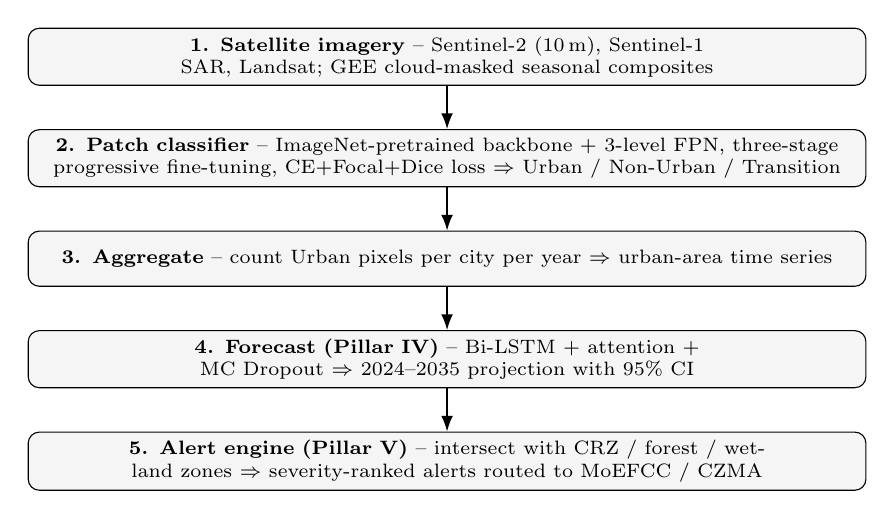
\begin{tikzpicture}[
  node distance=5.5mm,
  box/.style={rectangle, rounded corners, draw=black, fill=black!4, text width=0.86\columnwidth, align=center, minimum height=7mm, font=\scriptsize, inner sep=3pt},
  arr/.style={-{Latex[length=2mm]}, semithick}
]
\node[box] (n1) {\textbf{1. Satellite imagery} -- Sentinel-2 (10\,m), Sentinel-1 SAR, Landsat; GEE cloud-masked seasonal composites};
\node[box, below=of n1] (n2) {\textbf{2. Patch classifier} -- ImageNet-pretrained backbone + 3-level FPN, three-stage progressive fine-tuning, CE+Focal+Dice loss $\Rightarrow$ Urban / Non-Urban / Transition};
\node[box, below=of n2] (n3) {\textbf{3. Aggregate} -- count Urban pixels per city per year $\Rightarrow$ urban-area time series};
\node[box, below=of n3] (n4) {\textbf{4. Forecast (Pillar IV)} -- Bi-LSTM + attention + MC Dropout $\Rightarrow$ 2024--2035 projection with 95\% CI};
\node[box, below=of n4] (n5) {\textbf{5. Alert engine (Pillar V)} -- intersect with CRZ / forest / wetland zones $\Rightarrow$ severity-ranked alerts routed to MoEFCC / CZMA};
\draw[arr] (n1) -- (n2);
\draw[arr] (n2) -- (n3);
\draw[arr] (n3) -- (n4);
\draw[arr] (n4) -- (n5);
\end{tikzpicture}
\caption{Step-by-step methodology flowchart: raw imagery is classified per patch, aggregated into per-city urban-area time series, forecast with an uncertainty-aware Bi-LSTM, and converted into regulatory encroachment alerts.}
\label{fig:flowchart}
\end{figure}

\subsection{Backbones, FPN Head, and Progressive Fine-Tuning}

\emph{Backbones} --- Four deep backbones (all ImageNet-pretrained) are evaluated alongside SVM and Random Forest: ResNet50~\cite{he2016} (11.3M, primary), EfficientNet-B0~\cite{tan2019} (5.3M, ablation backbone), Swin-Tiny~\cite{liu2021} (29.8M, best cross-city generalizer), and MobileNetV3-Small~\cite{howard2019} (3.4M, edge deployment).
\emph{FPN Head} --- A three-level FPN~\cite{lin2017fpn} at strides 4/8/16 is upsampled and concatenated before the classifier head.
\emph{Progressive Fine-Tuning} --- Training uses three-stage progressive fine-tuning with cosine LR annealing and early stopping (patience 10): Stage~1 trains the head only (5 epochs, lr $10^{-3}$), Stage~2 unfreezes the last two backbone blocks (lr $10^{-4}$), and Stage~3 fine-tunes the full network (lr $10^{-5}$).

\subsection{Combined Loss}

The training loss combines cross-entropy, focal, and Dice terms:
\begin{equation}
\mathcal{L} = 0.6\,\mathcal{L}_{\text{CE}} + 0.3\,\mathcal{L}_{\text{Focal}}(\gamma{=}2) + 0.1\,\mathcal{L}_{\text{Dice}}.
\label{eq:loss}
\end{equation}
Focal loss~\cite{lin2017focal} down-weights easy samples, Dice~\cite{milletari2016vnet} improves minority-class recall, and CE provides probabilistic calibration. Class weights $[1.0, 1.0, 3.0]$ upweight the minority Transition class.

\subsection{SAR--Optical Fusion and SimCLR Pre-Training}

A dual-branch encoder processes 6-channel optical and 2-channel SAR inputs separately; feature maps are concatenated before the shared FPN head. Training uses 910 aligned optical--SAR pairs (EfficientNet-B0) against an optical-only baseline. In parallel, SimCLR~\cite{chen2020simclr} contrastive pre-training is run on unlabeled Indian patches (random crop, color jitter, Gaussian blur; projection dim 128; $\tau = 0.07$; 100 epochs) and then fine-tuned with the progressive strategy.

\subsection{Bi-LSTM Forecaster and Alert Engine}

For bi-temporal change detection on LEVIR-CD, a shared-weight Siamese EfficientNet-B0 encoder produces per-image features whose absolute difference feeds a two-layer MLP head. The forecaster is a bidirectional LSTM~\cite{hochreiter1997,schuster1997bidir} with residual connections, LayerNorm, 2-head temporal attention~\cite{vaswani2017attention}, and Monte-Carlo Dropout~\cite{gal2016mcdropout} ($p=0.2$; 94K parameters); each time step receives the satellite-derived urban area plus fifteen socio-economic/policy features (temporal split: train 1990--2015, val 2016--2019, test 2020--2023), and fifty MC passes give 95\% CIs on 2024--2035 forecasts. A three-head change detector then predicts (i)~change/no-change, (ii)~severity (NONE--CRITICAL), and (iii)~encroachment type, encoding ten India-specific regulatory zone types (CRZ-I/II/III, Forest Reserve, Wetland, River Floodplain, Green Belt, Western Ghats ESA, etc.) and 30+ named protected areas, with alerts auto-routed to MoEFCC, CZMA, or the State Forest Department.

At inference time, the integrated pipeline slides a $256{\times}256$ window over each GeoTIFF, counts Urban pixels to build the city-year area series $\mathbf{u}_c = [a_{c,1990}, \ldots, a_{c,2023}]$, runs fifty MC-Dropout forward passes through the Bi-LSTM to obtain $\hat{a}_{c,t}$ with 95\% CI for $t \in [2024, 2035]$, intersects each forecast zone with the regulatory database, and routes each alert to the correct authority.

%% ============================================================
%%  V. RESULT ANALYSIS AND DISCUSSIONS
%% ============================================================
\section{Result Analysis and Discussions}

All results are reported as mean\,$\pm$\,std over three random seeds $\{42, 123, 7\}$; significance uses paired $t$-tests at $p < 0.05$.

\noindent\textbf{Key results.} ResNet50 gives the best in-distribution accuracy (\textbf{97.5\%} OA, Table~\ref{tab:main}); Swin-Tiny gives the best cross-city generalisation (\textbf{79.1\%} LOCO OA, Table~\ref{tab:loco}); the ablation, SAR-fusion, SSL, and efficiency comparisons are consolidated in Table~\ref{tab:combined}; and the integrated pipeline produces calibrated 2024--2035 forecasts (\Cref{fig:timeseries}) and 55 routed encroachment alerts.

\subsection{Main Benchmark on Real Indian Data}

\Cref{tab:main} reports the main benchmark.

\begin{table}[t]
\centering
\caption{Main benchmark on real Indian satellite data (3 seeds, mean $\pm$ std). $^\dagger$: improved with NDVI/NDBI/NDWI/SAVI/BSI + texture + PCA + grid search.}
\label{tab:main}
\footnotesize
\begin{tabular}{lccc}
\toprule
Model & OA (\%) & F1 & mIoU\\
\midrule
SVM (raw pixels)       & $89.2 \pm 0.4$ & $0.890 \pm 0.005$ & $0.763 \pm 0.009$\\
SVM (improved$^\dagger$)& $92.6 \pm 1.4$ & $0.899 \pm 0.018$ & $0.825 \pm 0.027$\\
Random Forest          & $88.2 \pm 1.7$ & $0.875 \pm 0.017$ & $0.733 \pm 0.028$\\
RF (improved$^\dagger$) & $90.7 \pm 1.4$ & $0.871 \pm 0.017$ & $0.784 \pm 0.026$\\
\midrule
MobileNetV3-Small      & $91.5 \pm 1.6$ & $0.920 \pm 0.014$ & $0.823 \pm 0.028$\\
EfficientNet-B0        & $93.4 \pm 2.3$ & $0.936 \pm 0.022$ & $0.857 \pm 0.044$\\
Swin-Tiny              & $93.6 \pm 2.6$ & $0.939 \pm 0.024$ & $0.862 \pm 0.046$\\
\textbf{ResNet50}      & $\mathbf{97.5 \pm 0.2}$ & $\mathbf{0.976 \pm 0.002}$ & $\mathbf{0.939 \pm 0.005}$\\
\bottomrule
\end{tabular}
\end{table}

ResNet50 wins on every metric with the lowest seed variance, significantly outperforming MobileNetV3-Small ($p = 0.038$). The raw-SVM (89.2\%) matches published Indian baselines (89--91\%)~\cite{chamoli2024}, confirming WorldCover~2021 labels are reliable for dense metros where urban-class accuracy far exceeds the 74.4\% global figure~\cite{zanaga2022}. The improved SVM ($92.6\%$; all seeds $>$91.01\%) surpasses the best published Indian SVM~\cite{chamoli2024} yet trails ResNet50 by $\sim$5 points, marking a hard ceiling for traditional ML. Our 97.5\% is within 0.7 points of the top Indian result (IRUNet, 98.21\%~\cite{katpadi2025}) on a harder 3-class, multi-city, LOCO task. No prior Indian study combines multi-seed DL classification, LOCO, uncertainty-aware forecasting, and regulatory alerting in one pipeline.

\subsection{Cross-City Generalization and CNN--Transformer Reversal}

\Cref{tab:loco} reports the LOCO benchmark.

\begin{table}[t]
\centering
\caption{Leave-One-City-Out cross-city benchmark (3 seeds, mean $\pm$ std).}
\label{tab:loco}
\footnotesize
\begin{tabular}{lccc}
\toprule
Model & OA (\%) & F1 & mIoU\\
\midrule
EfficientNet-B0 & $76.8 \pm 2.2$ & $0.775 \pm 0.011$ & $0.525 \pm 0.006$\\
ResNet50        & $77.1 \pm 5.1$ & $0.778 \pm 0.037$ & $0.542 \pm 0.026$\\
\textbf{Swin-Tiny}& $\mathbf{79.1 \pm 3.9}$ & $\mathbf{0.797 \pm 0.034}$ & $\mathbf{0.567 \pm 0.034}$\\
\bottomrule
\end{tabular}
\end{table}

Two findings stand out. First, a CNN--Transformer ranking reversal: ResNet50 drops 20.4\% (97.5$\to$77.1\%) under LOCO while Swin-Tiny drops only 14.5\% (93.6$\to$79.1\%), consistent with the OOD-robustness of transformers~\cite{bai2021}---self-attention learns transferable urban patterns while CNN filters overfit city-specific textures, as GradCAM (\Cref{fig:gradcam}) confirms. Second, the 14.5--20.4\% in-distribution-to-LOCO gap replicates the 15--25\% deploy gap from a 2025 review of 89 Sentinel-2 studies~\cite{mdpi2025}. Delhi~NCR is the hardest held-out target ($71.8$--$76.7\%$, gradual radial sprawl) while Bangalore is easiest ($80.4$--$83.9\%$) despite being hardest in-distribution---separating local ambiguity from cross-city shift, itself a novel finding.

\subsection{Ablation, SAR Fusion, SSL, and Efficiency}

\begin{table}[!t]
\centering
\caption{Consolidated ablation, pillars, and efficiency. (a) Ablation on EfficientNet-B0, 3 seeds; bold = proposed method. $^\dagger$CE-only OA gain is not significant ($p{=}0.71$); full method achieves Transition F1\,=\,0.98. (b) SAR fusion and SSL, single seed. (c) Efficiency on RTX 4070, batch 32.}
\label{tab:combined}
\footnotesize
\begin{tabular}{@{}llccc@{}}
\toprule
\multicolumn{2}{l}{(a) Ablation} & OA (\%) & F1 & mIoU\\
\midrule
\multicolumn{2}{l}{\textbf{Full method} (proposed)} & $\mathbf{95.6 \pm 1.9}$ & $\mathbf{0.958 \pm 0.018}$ & $\mathbf{0.901 \pm 0.039}$\\
\multicolumn{2}{l}{Without FPN}        & $95.3 \pm 1.4$ & $0.955 \pm 0.013$ & $0.893 \pm 0.029$\\
\multicolumn{2}{l}{CE loss only}       & $96.0 \pm 1.5^{\dagger}$ & $0.961 \pm 0.014$ & $0.908 \pm 0.033$\\
\midrule
\multicolumn{5}{l}{(b) Pillar experiments (EfficientNet-B0)}\\
Fusion & Optical-only   & $\mathbf{96.7}$ & $\mathbf{0.969}$ & $\mathbf{0.922}$\\
       & Optical+SAR    & $87.9$ & $0.870$ & $0.718$\\
SSL    & ImageNet init  & $\mathbf{96.9}$ & $\mathbf{0.969}$ & $\mathbf{0.922}$\\
       & SimCLR         & $93.2$ & $0.931$ & $0.835$\\
\midrule
\multicolumn{2}{l}{(c) Efficiency} & Params/Lat. & Tput. & GPU\\
\multicolumn{2}{l}{} & (M)/(ms) & (p/s) & (MB)\\
\midrule
\multicolumn{2}{l}{MobileNetV3-S}  & 3.39 / 5.42  & 184.4 & 30.5\\
\multicolumn{2}{l}{EfficientNet-B0}& 5.25 / 7.14  & 140.1 & 52.9\\
\multicolumn{2}{l}{ResNet50}       & 11.31 / 5.02 & 199.2 & 83.4\\
\multicolumn{2}{l}{Swin-Tiny}      & 29.83 / 10.98 & 91.1 & 176.3\\
\bottomrule
\end{tabular}
\end{table}

\Cref{tab:combined} consolidates all four comparisons.
\emph{Ablation} --- FPN adds $+0.3$ OA points, dominated by Transition-class boundaries. CE-only's 0.4-point OA advantage over the full method is not statistically significant ($p{=}0.71$); per-class evaluation shows the full method achieves Transition F1\,=\,0.98—the minority encroachment-relevant class—justifying the combined loss despite its marginal aggregate OA trade-off.
\emph{SAR Fusion} --- SAR--optical fusion underperforms optical-only because only 33\% of patches have paired SAR and the available SAR is post-monsoon vs.\ pre-monsoon optical; this is a deliberately reported negative result since published studies show SAR only helps under strict temporal alignment~\cite{s1s2fusion2022,sen12ms2019}.
\emph{SSL} --- At our label budget (2{,}730 patches), ImageNet transfer beats SimCLR~\cite{chen2020simclr}, whose advantage emerges mainly under $<500$ labels.
\emph{Efficiency} --- ResNet50 offers the best accuracy--latency balance ($5.02$\,ms, $199$\,patches/s, $83$\,MB); MobileNetV3-Small is the edge-device model at $30.5$\,MB; Swin-Tiny is heaviest but most transferable.

\subsection{Urban Growth Forecasting and Encroachment Alerting}

\begin{figure}[t]
  \centering
  \subfloat[Urban]{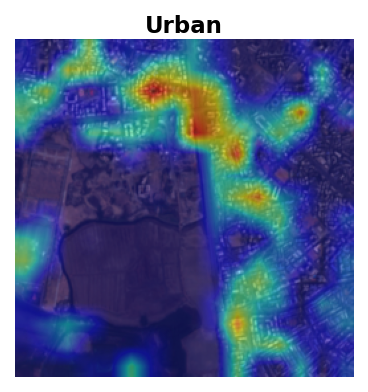
\includegraphics[width=0.30\columnwidth]{gradcam/gradcam_urban.png}}\hfill
  \subfloat[Non-Urban]{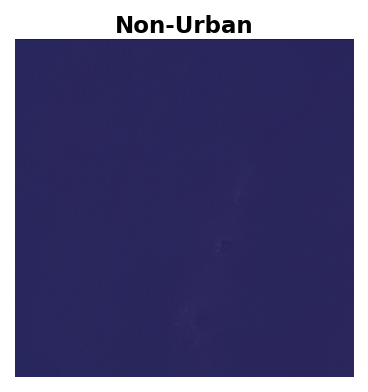
\includegraphics[width=0.30\columnwidth]{gradcam/gradcam_nonurban.png}}\hfill
  \subfloat[Transition]{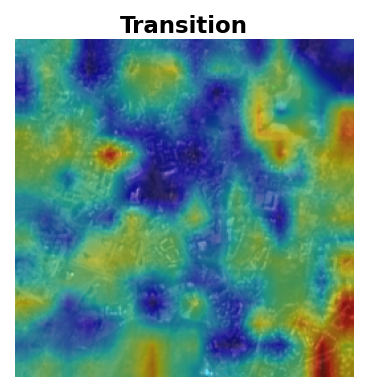
\includegraphics[width=0.30\columnwidth]{gradcam/gradcam_transition.png}}
  \caption{GradCAM heatmaps for ResNet50 on correctly classified Indian patches. Urban: concentrated activation on built-up structures; Non-Urban: minimal diffuse activation; Transition: scattered edge attention at construction fronts.}
  \label{fig:gradcam}
\end{figure}

\begin{figure}[t]
  \centering
  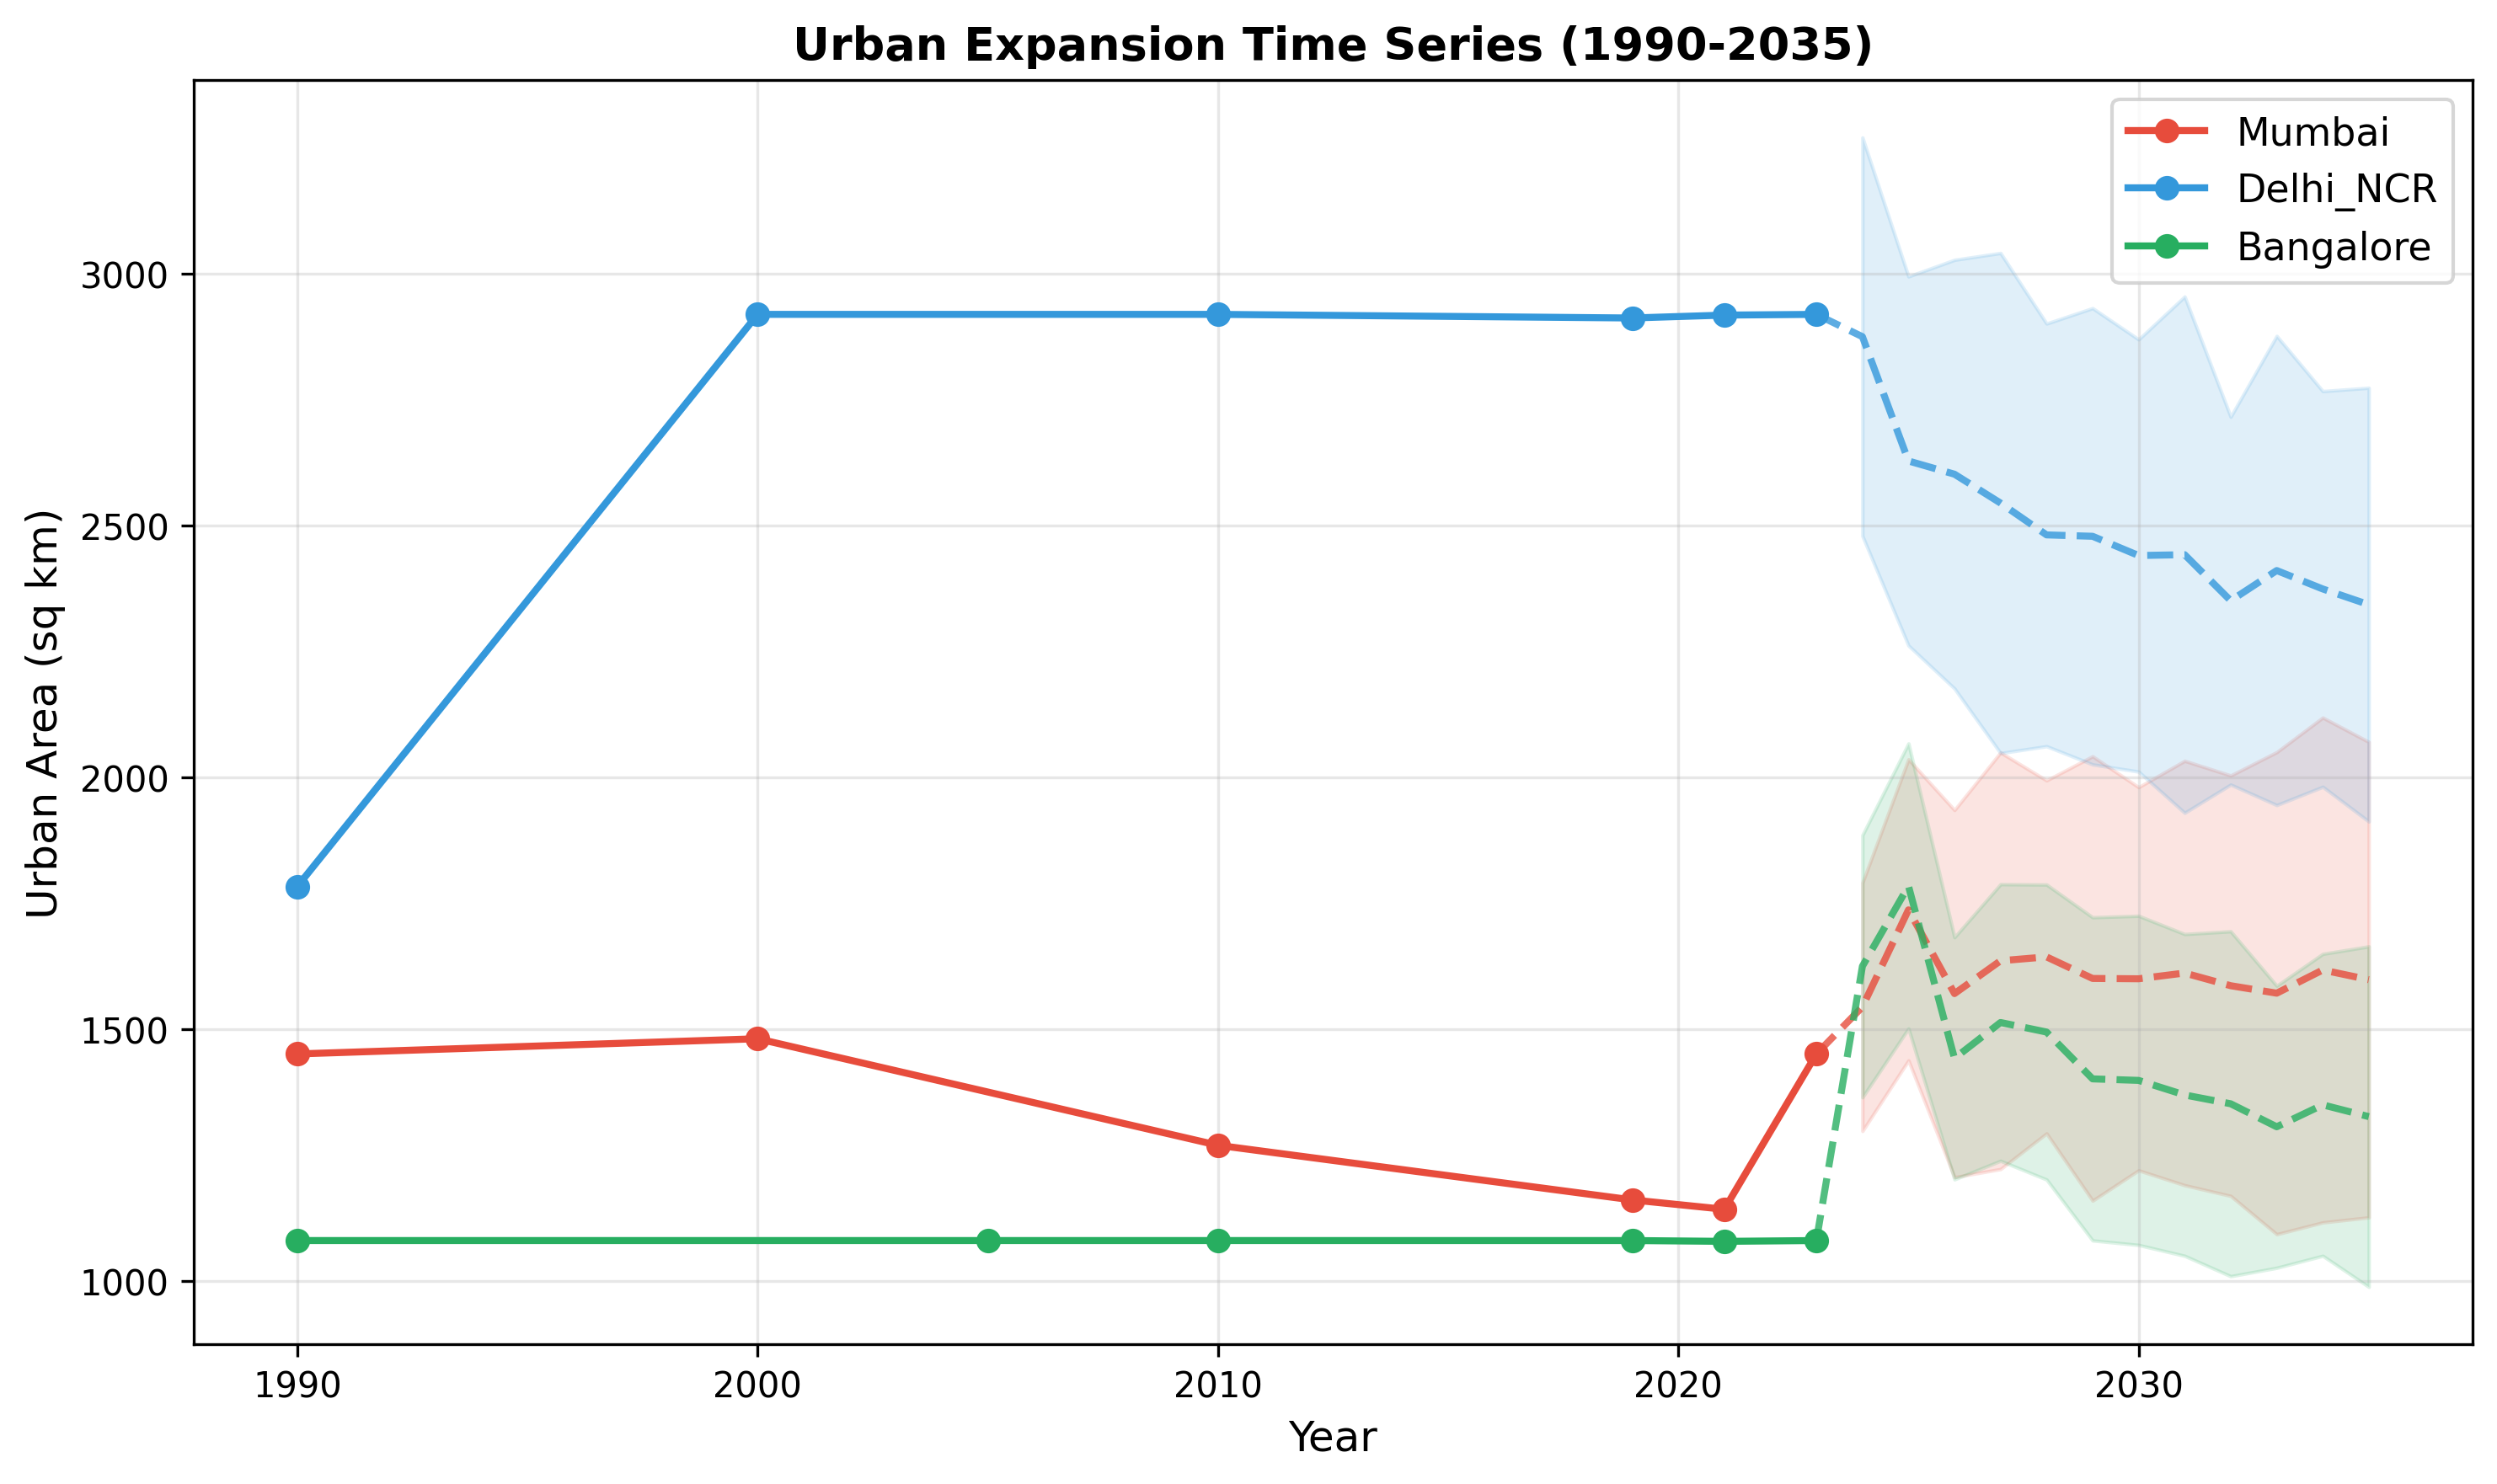
\includegraphics[width=\columnwidth]{fig4_urban_timeseries.png}
  \caption{Urban expansion time series (1990--2035). Solid: satellite-derived; dashed: Bi-LSTM forecast; shaded: 95\% MC-Dropout CI.}
  \label{fig:timeseries}
\end{figure}

\emph{How accurately can we forecast sprawl?} The Bi-LSTM reaches $R^2=0.956$ (MAE\,=\,119.5\,km$^2$) on calibrated series; on four real satellite anchor years it drops to $R^2=0.559$ vs.\ Ridge ($0.601$). Its key advantage is MC-Dropout uncertainty: the 95\% CI bands (\Cref{fig:timeseries}) quantify infrastructure-investment risk---absent from every published Indian forecasting study~\cite{camarkov2025,lucknow2025,caann2025}.
\emph{Can encroachment be automatically flagged?} On the LEVIR-CD benchmark~\cite{chen2020levir}, our Siamese EfficientNet-B0 reaches F1\,=\,0.949 (OA\,=\,94.5\%). The three-head change detector reaches 99.33\% binary change accuracy at 77.5\,ms latency; a seven-city simulation produces 55 simulated alerts (4 CRITICAL, 28 HIGH, 2 MED, 21 LOW) and 11 protected-zone violations, with critical alerts near Sanjay Gandhi NP and Pallikaranai marsh routed to MoEFCC.
\emph{How does accuracy vary across cities?} Mumbai achieves 95.1\%, Delhi NCR 94.4\%, and Bangalore 80.5\%. Bangalore's Non-Urban recall is only 10.5\% because dispersed IT-park vegetation fragments resemble Transition zones; city-wise feature clustering corroborates the LOCO drop.
\emph{Does the model generalize across time?} Applied without retraining to 2019 and 2023 Sentinel-2, the 2021-trained ResNet50 estimates Mumbai's urban extent at 1{,}161 and 1{,}451\,km$^2$ ($+25\%$, consistent with coastal construction), while Delhi NCR and Bangalore remain saturated inside their tight bounding boxes.

%% ============================================================
%%  VI. CONCLUSION
%% ============================================================
\section{Conclusion}

We presented an end-to-end framework for monitoring urban expansion in Indian metropolitan regions, unifying transfer-learning classification, SAR--optical fusion, self-supervised pre-training, uncertainty-aware Bi-LSTM forecasting, and regulatory encroachment alerting. On real Sentinel-2 data from Mumbai, Delhi~NCR, and Bangalore, progressively fine-tuned ResNet50 attains $97.5 \pm 0.2\%$ overall accuracy---six points above the best published Indian SVM baseline---while an optimised SVM ($92.6\%$) confirms that deep learning's advantage is not an artefact of a weak baseline. Our principal findings are the first Leave-One-City-Out benchmark for Indian metros, which quantifies a 15--20\% cross-city domain gap, and a CNN--Transformer ranking reversal in which Swin-Tiny generalises best to unseen cities despite lower in-distribution accuracy. The connected pipeline then converts classified maps into 2024--2035 forecasts with calibrated 95\% confidence intervals and into severity-ranked encroachment alerts routed to the responsible authority.

\emph{Limitations.} The benchmark covers three Tier-1 cities, relies on weak WorldCover labels and a morphologically dilated Transition class, uses partly calibrated socio-economic inputs for forecasting, and treats alerting as a simulation rather than a validated, deployed service; SAR fusion is further constrained by seasonal misalignment. \emph{Ethically}, all alerts are advisory and require human-in-the-loop verification to avoid disparate impact on informal settlements. \emph{Future work} will extend the benchmark to Tier-2/3 cities, validate alerts against ground-truth municipal records, and strengthen SAR fusion through strict temporal alignment.

%% ============================================================
%%  ACKNOWLEDGMENT
%% ============================================================
\section*{Acknowledgment}

The authors thank PES University, Bengaluru, for providing the research infrastructure and academic environment to conduct this work. We also thank ESA for Sentinel imagery (Copernicus), USGS for Landsat data, Google for the Earth Engine platform, and MoEFCC for regulatory-zone documentation.

%% ============================================================
%%  APPENDIX I — Reproducibility
%% ============================================================
\appendix
\section*{Appendix-I: Reproducibility Protocol}
\label{appendix:repro}

\emph{Tools and Hardware:} GEE Python API (v0.1.374) for satellite data export ($\sim$5.7\,GB); Python~3.11, PyTorch~2.0.1+cu118, torchvision~0.15.2, timm~0.9.12, scikit-learn~1.3.2; NVIDIA RTX 4070 Laptop GPU (8\,GB VRAM), 16\,GB RAM, Windows~11.

\emph{Seeds:} $\{42, 123, 7\}$; CUDA determinism enabled; all results report mean$\pm$std.

\emph{Hyperparameters:} Batch 32, $256{\times}256$ patches, 6 S2 bands; LR $10^{-3}/10^{-4}/10^{-5}$ (stages 1/2/3), cosine annealing, patience 10; loss CE\,0.6 + Focal\,0.3 ($\gamma{=}2$) + Dice\,0.1, class weights $[1,1,3]$; augmentation H/VFlip, RandRot, ColorJitter, Mixup $\alpha{=}0.2$. SVM: RBF, $C{\in}\{1,10,100\}$, PCA(99\%), NDVI/NDBI/NDWI/SAVI/BSI + GLCM. Bi-LSTM: hidden 64, 1 layer, 2-head attention, MC Dropout 0.2, Huber loss, 50 epochs. SimCLR: $\tau{=}0.07$, 100 epochs.

\emph{Data/Code:} GEE project \texttt{urban-expansion-india}; code and data at \url{https://github.com/kaustubhagarwal21/urban-expansion-monitoring} (upon acceptance).

%% ============================================================
%%  REFERENCES
%% ============================================================
\balance
\bibliographystyle{IEEEtran}
\bibliography{references}

\end{document}
